\subsection{CentralServer}
Ifm. unit-testing af CentralServer er der lagt vægt på at designe systemet således, at unit-testing er muligt. Det betyder, at klasser så vidt muligt bør afhænge af interfaces frem for konkrete implementeringer.\\

Det skal siges, at CentralServer benytter discipliner som gør det meget omfattende at unit-teste bestemte klasser. Her refereres til multitrådet programmering, sockets samt database. Der er derfor lagt vægt på, at unit-teste klasser, som ikke afhænger af disse discipliner.\\

Der er benyttet nunit og nsubstitute til at udføre unit-testene.


	\begin{figure}[H]
		\centering
		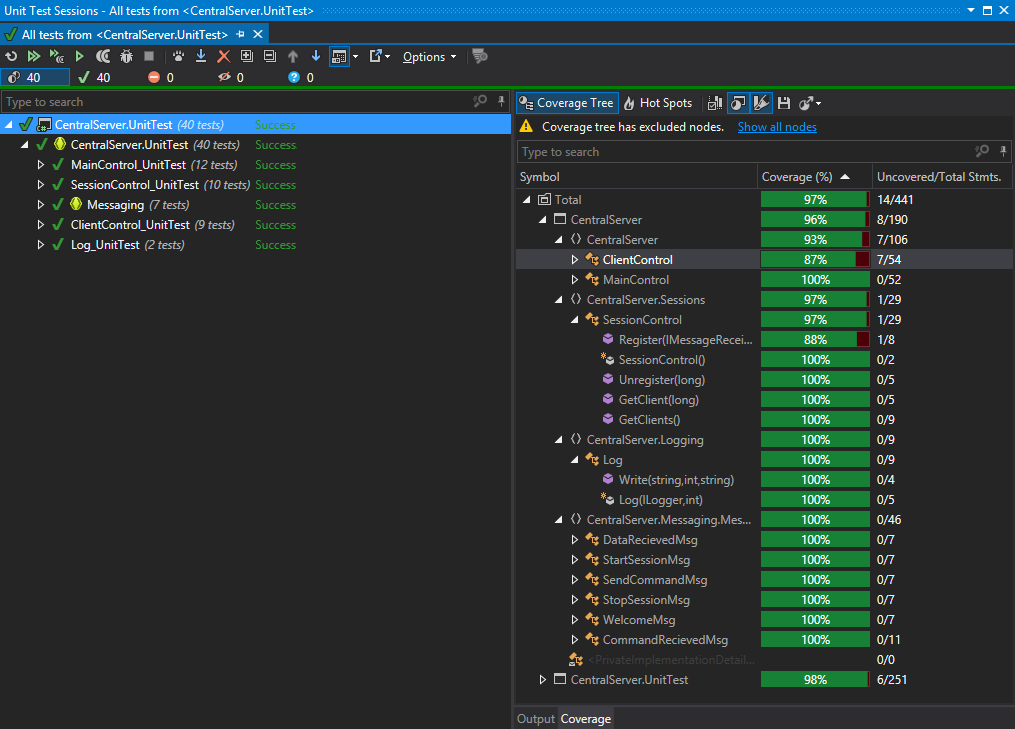
\includegraphics[width=1\textwidth]{Test/Images/CentralServer_unittest.png}
		\caption{Antal unit tests samt coverage for CentralServer}
		\label{fig:antalunit}
	\end{figure}